\documentclass{standalone}
\usepackage[usenames,dvipsnames]{xcolor}
\usepackage{amsmath, amssymb, amsthm}

\usepackage{tikz}
\begin{document}
	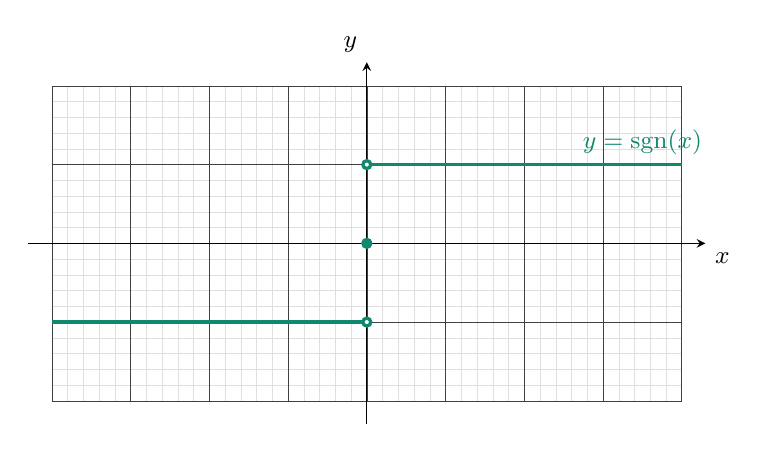
\begin{tikzpicture}[font=\small]
		\draw[step=0.2cm, gray!25,very thin] (-4,-2) grid (4,2);
		\draw[step=1cm, black!75,very thin] (-4,-2) grid (4,2);
		\draw[-stealth] (-4.3,0) -- (4.3,0) node [below right] {$x$};
		\draw[-stealth] (0,-2.3) -- (0,2.3) node [above left] {$y$};
		\draw[very thick,color=PineGreen] plot[domain=0:4] (\x, 1); 
		\draw[very thick,color=PineGreen] plot[domain=-4:0] (\x, -1);
		\draw[very thick,color=PineGreen, fill=PineGreen] (0,0) circle (0.05cm); 
		\draw[very thick,color=PineGreen, fill=white] (0,1) circle (0.05cm); 
		\draw[very thick,color=PineGreen, fill=white] (0,-1) circle (0.05cm); 
		\draw[color=PineGreen] (3.5,1) node [above] {$y=\text{sgn}(x)$};
	\end{tikzpicture}
\end{document}